% 
% This message contains the LaTeX template for scribe notes
% in EE597.  You are free to use other means of producing
% your notes, but you are encouraged to use LaTeX: you will
% need to learn it some day.
% 
% Many thanks to Alistair Sinclair@cs.berkeley.edu for providing the basis for
% the first version of this template.
% 
% %************************************************************
%
% This is the LaTeX template file for lecture notes for EE596
% Pattern Recognition II: Introduction to Graphical Models.  When preparing 
% LaTeX notes for this class you must use this template.
%
% To familiarize yourself with this template, the body contains
% some examples of its use.  Look them over.  Then you can
% run LaTeX on this file.  After you have LaTeXed this file then
% you can look over the result either by printing it out with
% dvips or using xdvi.
%

\documentclass{article}
\usepackage{times,amsmath,amsthm,amsfonts,eucal,graphicx,tikz,fixltx2e,mathtools,tkz-berge}

% This scribe template not only uses latex, but also
% the American Mathematical Society (AMS) latex macros.
% Detailed documentation on how to use them to produce good
% math formating can be obtained here: http://www.ams.org/tex/
% I've also placed a copy of the AMS-Latex documentation
% on the web page at:
%     http://www.ee.washington.edu/class/596/patrec/scribes/amsguide_2p.ps
% Latex documentation can be obtained from 
%
% Publications related to latex are listed here:
%     http://www.ams.org/tex/publications.html
%

\setlength{\oddsidemargin}{0.25 in}
\setlength{\evensidemargin}{-0.25 in}
\setlength{\topmargin}{-0.6 in}
\setlength{\textwidth}{6.5 in}
\setlength{\textheight}{8.5 in}
\setlength{\headsep}{0.75 in}
\setlength{\parindent}{0 in}
\setlength{\parskip}{0.1 in}

%
% The following commands set up the lecnum (lecture number)
% counter and make various numbering schemes work relative
% to the lecture number.
%
\newcounter{lecnum}
\renewcommand{\thepage}{\thelecnum-\arabic{page}}
\renewcommand{\thesection}{\thelecnum.\arabic{section}}
\renewcommand{\theequation}{\thelecnum.\arabic{equation}}
\renewcommand{\thefigure}{\thelecnum.\arabic{figure}}
\renewcommand{\thetable}{\thelecnum.\arabic{table}}

%
% A few symbols that we will be using often in this course.
\newcommand{\indep}{{\bot\negthickspace\negthickspace\bot}}
\newcommand{\notindep}{{\not\negthickspace\negthinspace{\bot\negthickspace\negthickspace\bot}}}
\newcommand{\definedtobe}{\stackrel{\Delta}{=}}
\renewcommand{\choose}[2]{{{#1}\atopwithdelims(){#2}}}
\newcommand{\argmax}[1]{{\hbox{$\underset{#1}{\mbox{argmax}}\;$}}}
\newcommand{\argmin}[1]{{\hbox{$\underset{#1}{\mbox{argmin}}\;$}}}

%
% The following macro is used to generate the header.
%
\newcommand{\lecture}[4]{
   \pagestyle{myheadings}
   \thispagestyle{plain}
   \newpage
   \setcounter{lecnum}{#1}
   \setcounter{page}{1}
   \noindent
   \begin{center}
   \framebox{
      \vbox{\vspace{2mm}
    \hbox to 6.58in { {\bf CS502: Graph Theory and Applications
                        \hfill Fall 2019-20} }
    \hbox to 6.58in { {\bf 
                        \hfill } }
       \vspace{4mm}
       \hbox to 6.28in { {\Large \hfill Lecture #1: #2  \hfill} }
       \vspace{2mm}
       \hbox to 6.28in { {\it Instructor: {\it Vinod Reddy} \hfill Scribe: #3} }
      \vspace{6mm}}
   }
   \end{center}
   \markboth{Lecture #1 #2}{Lecture #1 #2}
   \vspace*{4mm}
}

%
% Convention for citations is authors' initials followed by the year.
% For example, to cite a paper by Leighton and Maggs you would type
% \cite{LM89}, and to cite a paper by Strassen you would type \cite{S69}.
% (To avoid bibliography problems, for now we redefine the \cite command.)
% Also commands that create a suitable format for the reference list.
\renewcommand{\cite}[1]{[#1]}
\def\beginrefs{\begin{list}%
        {[\arabic{equation}]}{\usecounter{equation}
         \setlength{\leftmargin}{2.0truecm}\setlength{\labelsep}{0.4truecm}%
         \setlength{\labelwidth}{1.6truecm}}}
\def\endrefs{\end{list}}
\def\bibentry#1{\item[\hbox{[#1]}]}

%Use this command for a figure; it puts a figure in wherever you want it.
%usage: \fig{NUMBER}{CAPTION}{.eps FILE TO INCLUDE}{WIDTH-IN-INCHES}
\newcommand{\fig}[4]{
			\begin{center}
	                \includegraphics[width=#4,clip=true]{#3} \\
			Figure \thelecnum.#1:~#2
			\end{center}
	}
% Use these for theorems, lemmas, proofs, etc.
\newtheorem{theorem}{Theorem}[lecnum]
\newtheorem{lemma}[theorem]{Lemma}
\newtheorem{proposition}[theorem]{Proposition}
\newtheorem{claim}[theorem]{Claim}
\newtheorem{corollary}[theorem]{Corollary}
\newtheorem{definition}[theorem]{Definition}
% \newenvironment{proof}{{\bf Proof:}}{\hfill\rule{2mm}{2mm}}

% **** IF YOU WANT TO DEFINE ADDITIONAL MACROS FOR YOURSELF, PUT THEM HERE:

\begin{document}
%FILL IN THE RIGHT INFO.
%\lecture{**LECTURE-NUMBER**}{**DATE**}{**LECTURER**}{**SCRIBE**}
\lecture{1}{Basics of Graph Theory}{GVN Sai Uday(11740320) \& E Suyra Teja(11740310)} %\hfill\break\qquad E Suyra Teja(11740310)}
%\footnotetext{These notes are partially based on those of Nigel Mansell.}

% **** YOUR NOTES GO HERE:

% Some general latex examples and examples making use of the
% macros follow.  
%**** IN GENERAL, BE BRIEF AND COMPLETE. 
In this lecture, we will be dealing with some basic terminology
required to learn Graph Theory.\\%~\\

\quad A graph G is a pair $G=(V,E)$, where V is a finite set and E is a set of 2-element subsets of V. 
The elements of V are called vertices of the graph G and the elements of E are called edges of G.\\

\quad For a graph $G=(V,E)$, let $V(G)$ \& $E(G)$ denote the vertex and edge set of G respectively.

\textbf{Example:-}
\begin{center}
\begin{tikzpicture}[auto,node distance=3cm,
                    thick,main node/.style={circle,draw,font=\sffamily\bfseries}]

  \node[main node] (1) {1};
  \node[main node] (2) [right of=1] {2};
  \node[main node] (3) [below right of=2] {3};
  \node[main node] (4) [below left of=2] {4};

  \path[every node/.style={font=\sffamily\small}]
    (1) edge node [left] {} (4)
    (2) edge node [right] {} (1)
        edge node {} (4)
    (3) edge node [right] {} (2);
\end{tikzpicture}
\end{center}

$$ V = \{1,2,3,4\} $$ \\[-1cm] $$ E = \{\{1,2\},\{1,4\},\{2,3\},\{2,4\}\}$$

\quad The number of vertices of a graph G is its order(or size), denoted as $|G|$ or $|V|$.

\textbf{Note}:- 
\begin{itemize}
\item From this lecture onwards \emph{n} denotes the number of vertices in a graph.
\item Also \emph{m} denotes the number of edges in a graph.
\item The graphs we consider in this course are finite
unless otherwise stated.
\end{itemize}

\quad An edge ${x,y}$ is usually written as $xy$ (or $yx$). 
Two vertices ${x,y}$ of G are adjacent or neighbours if $xy$ is an edge of G. 
Two edges $e,f$ are adjacent if they have an end in common.

\begin{definition}[Degree(or Valency)]
\quad The \emph{degree(or valency)} of a vertex $v$ in a graph G is the number of edges incident with $v$, 
with loops counted twice. It is denoted by deg\textsubscript{G}($v$) or d($v$).\\~\\~\\
\end{definition}

\begin{lemma}[Handshaking Lemma]
The sum of the degrees of the vertices of a graph equals twice the number of edges.
\end{lemma}

\begin{proof}
Each edge contributes two to the sum of the degrees, one for each of its endpoints.
$$ 2|E| = \sum_{v \epsilon V} d(v)$$\\
\end{proof}

\begin{corollary}
In any graph G, the number of vertices of odd degree is even.
\end{corollary}

\begin{proof}
We know that
$$ 2|E| = \sum_{v \epsilon V} d(v)$$\\
$$ \underbrace{2|E|}_\text{\clap{EVEN~}} = 
\underbracket{\sum_{\substack{v \epsilon V\\d(v) is odd}} d(v)}_\text{\clap{\textbf{x~}}} 
+ \underbracket{\sum_{\substack{v \epsilon V\\d(v) is even}} d(v)}_\text{\clap{EVEN~}} $$\\
\quad For the above equation to satisfy the value of \textbf{x} should be even(i.e. for the LHS 
to be even sum of terms of RHS should be even, which is only possible when value of \textbf{x}
is even since the other term is even.)
\end{proof}

\begin{definition}[Isolated vertex]
\quad A vertex of degree zero is called isolated vertex.\\
\end{definition}

\begin{definition}[Minimum degree]
\quad The degree of the vertex with the least number of edges incident to it 
(i.e. $min\{d(v) : v \epsilon V\}$) is the minimum degree of G.
It is represented by $\delta(G)$\\
\end{definition}

\begin{definition}[Maximum degree]
\quad The degree of the vertex with the most number of edges incident to it 
(i.e. $max\{d(v) : v \epsilon V\}$) is the maximum degree of G.
It is represented by $\Delta(G)$\\
\end{definition}

\begin{definition}[Regular Graph]
\quad If all the vertices of G have the same degree k then the graph G is called k-regular.\\
\end{definition}

\textbf{Example:-}\\
\textbf{(a) 2-Regular Graph}\\
\begin{center}
\begin{tikzpicture}[auto,node distance=3cm,
                    thick,main node/.style={circle,draw,font=\sffamily\bfseries}]

  \node[main node] (1) {1};
  \node[main node] (2) [right of=1] {2};
  \node[main node] (3) [below of=2] {3};
  \node[main node] (4) [below of=1] {4};

  \path[every node/.style={font=\sffamily\small}]
    (1) edge node [left] {} (4)
    (2) edge node [right] {} (1)
    (3) edge node [right] {} (2)
    (4) edge node [left] {} (3); 
\end{tikzpicture}
\end{center}

\textbf{(b) Petersen's Graph(3-Regular Graph)}\\
\begin{center}
\begin{tikzpicture}[scale=0.6]
\grPetersen[form=1,RA=5,RB=3]
\end{tikzpicture}
\end{center}

\textbf{(c) 3-Regular Graph}\\
\begin{center}
\begin{tikzpicture}[auto,node distance=3cm,
                    thick,main node/.style={circle,draw,font=\sffamily\bfseries}]

  \node[main node] (1) {1};
  \node[main node] (2) [below left of=1] {2};
  \node[main node] (3) [below right of=2] {3};
  \node[main node] (4) [below of=1] {4};

  \path[every node/.style={font=\sffamily\small}]
    (1) edge node [left] {} (4)
    (2) edge node [right] {} (1)
    (3) edge node [right] {} (2)
    (4) edge node [left] {} (3);
\end{tikzpicture}
\end{center}

\section{Some theorems and stuff} % Don't be this informal in your notes!

We now delve right into the proof.

\begin{lemma}
This is the first lemma of the lecture.
\end{lemma}

\begin{proof}
The proof is by induction on \ldots.
We also throw in a figure (which you might want to make larger).
%%%NOTE USAGE !

%\fig{1}{A Figure}{six-node-example}{1.5in}

This is the end of the proof, which is marked with a little box.
\end{proof}

\subsection{A few items of note}

Here is an itemized list:
\begin{itemize}
\item this is the first item;
\item this is the second item.
\end{itemize}
Here is an enumerated list:
\begin{enumerate}
\item this is the first item;
\item this is the second item.
\end{enumerate}

Here is an exercise:

{\bf Exercise:}  Find an efficient algorithm for triangulation.

Here is how to define things in the proper mathematical style.
Let $f_k$ be the $AND-OR$ function, defined by

\[ f_k(x_1, x_2, \ldots, x_{2^k}) = \left\{ \begin{array}{ll}

	x_1 & \mbox{if $k = 0$;} \\

	\mbox{AND}(f_{k-1}(x_1, \ldots, x_{2^{k-1}}),
	   f_{k-1}(x_{2^{k-1} + 1}, \ldots, x_{2^k}))
	 & \mbox{if $k$ is even;} \\

	\mbox{OR}(f_{k-1}(x_1, \ldots, x_{2^{k-1}}),
	   f_{k-1}(x_{2^{k-1} + 1}, \ldots, x_{2^k}))	
	& \mbox{otherwise.} 
	\end{array}
	\right. \]

Here is another equation that uses one of the AMS commands, align
{\small 
\begin{align*}
p(x_{1:5}) & = 
\sum_{x_{2:5}} 
p(x_1)p(x_2|x_1)p(x_3|x_1)p(x_4|x_2)
p(x_5|x_1)p(x_6|x_2,x_5) \\
& =  
p(x_1)\sum_{x_2}p(x_2|x_1)\sum_{x_3}p(x_3|x_1)\sum_{x_4}p(x_4|x_2)
\sum_{x_5}p(x_5|x_1)p(x_6|x_2,x_5) \\
& =  
p(x_1)\sum_{x_2}p(x_2|x_1)\sum_{x_3}p(x_3|x_1)\sum_{x_4}p(x_4|x_2)
\sum_{x_5}p(x_5|x_1)\phi_{X_6}(x_2,x_5)
\end{align*}
}
which assumes that $X_4 \indep \{ X_1, X_3 \} | X_2$.

\begin{theorem}
This is the first theorem.
\end{theorem}

\begin{proof}
This is the proof of the first theorem. We show how to write pseudo-code now.
%*** USE PSEUDO-CODE ONLY IF IT IS CLEARER THAN AN ENGLISH DESCRIPTION

Consider a comparison between $x$ and~$y$:
\begin{tabbing}
\hspace*{.25in} \= \hspace*{.25in} \= \hspace*{.25in} \= \hspace*{.25in} \= \hspace*{.25in} \=\kill
\>{\bf if} $x$ or $y$ or both are in $S$ {\bf then } \\
\>\> answer accordingly \\
\>{\bf else} \\
\>\>    Make the element with the larger score (say $x$) win the comparison \\
\>\> {\bf if} $F(x) + F(y) < \frac{n}{t-1}$ {\bf then} \\%
\>\>\> $F(x) \leftarrow F(x) + F(y)$ \\
\>\>\> $F(y) \leftarrow 0$ \\
\>\> {\bf else}  \\
\>\>\> $S \leftarrow S \cup \{ x \} $ \\
\>\>\> $r \leftarrow r+1$ \\
\>\> {\bf endif} \\
\>{\bf endif} 
\end{tabbing}

This concludes the proof.
\end{proof}

\section{Next topic}

Here is some citations \cite{JB00} and \cite{L2000}

\section*{References}
\beginrefs
\bibentry{JB00}{\sc M.I.~Jordan} and {\sc C.~Bishop}, 
``An Introduction to Graphical Models,''
{\it To be published},
2000

\bibentry{L2000}{\sc S.L.~Lauritzen}
``Graphical Models,''
{\it Oxford Science Publications},
1996



\endrefs

% **** THIS ENDS THE EXAMPLES. DON'T DELETE THE FOLLOWING LINE:

\end{document}


